\documentclass[a4paper,10pt]{article}
\usepackage{graphicx}
\usepackage[english]{babel}
\usepackage[latin1]{inputenc}
\usepackage{cite}
\usepackage{hyperref}
\usepackage[table]{xcolor}
\usepackage{geometry}

\geometry{margin=1in} % Adjust margins as needed
%
\begin{document}
%
  \title{Animal Image Classification}
  \author{
  Isaiah Martinez \\ CSUN \\ Computer Science Department \\ isaiah.martinez.891@my.csun.edu
  \and
  Joycelyn Tuazon \\ CSUN \\ Computer Science Department \\ joycelyn.tuazon.251@my.csun.edu}
          
  \date{12/02/2023}

  \maketitle
   
  \tableofcontents
 
  % to import a new page into this document, use
  % `\include{FILENAME}`
  %     Note: FILENAME does NOT include the `.tex` file extension
  % compilation follows as normal

  \newpage

  \section{Introduction}
[Background on the topic]

\begin{enumerate}
\item In the first section we will describe the process toward which the results of the project were obtained.
\item The section presents the results we obtained with...
\end{enumerate}

The introduction should state clearly why the study was started
and give a relatively short and essential overview of the topic
you are exploring. References to previous works can be made here.
 
The introduction should not contain the conclusions. 
At the end of the introduction the outline of the paper may be described.


(Problem)
We wanted to learn more about using Machine Learning techniques in Image Classification.

(Dataset + Description)
Cat, Dog, Panda of RGB images of sizes. Simple metrics and dataset size.

(Data Preparation)
RGB, Grayscale, into array, sizing

(Data Visualization)
Insert sample image (1-2) + conversion to array
How did conversion work for each case


  \graphicspath{ {project_images/} }
\section{Related Works}

\subsection{SVM}
The first algorithm we looked at was Support Vector Machine (SVM) Classifier. 
Initial Research done showed that SVM outperformed Naive Bayes when perfoming image classification \cite{SVM}.
Through the use of Pipeline and Grid Search, we were able to find optimal performing parameters including: kernel, C, and gamma.
Grid Search allowed us to perform K-Fold cross validation on the model so that we would obtain more stable results.

\subsection{CNN}
Convolutional Neural Networks (CNN) were the main types of algorithms used by others looking into Image Classification.
This is because previous studies have shown the advantages to using such models to analyze and predict based on such complex datasets \cite{CNNPerformance}.
Additionally, there are various works using CNN models to perform varying types of Image Classification for several animals including primates, rodents, canines, felines, aves, and insecta \cite{AnimalSpecies1, AnimalSpecies2, AnimalBreed, Mosquito}.
When constructing our CNN models, we used the ReLu activation function for each hidden layer as well as the Adam optimizer since this seemed to be a common practice to improve performance.

\subsection{VGG16}
The VGG16 algorithm was particularly interesting to us because it is available for use as a pre-trained model.
There is one work in particular that conducted an experiment that involved using the pre-trained VGG16 model to classify greyscale images of dogs and cats \cite{VGG16Greyscale}. We had discussed the possibility of converting our dataset to greyscale images to potentially reduce computational load. We did end up converting our images to greyscale and this article confirmed that it would be possible to train the VGG16 model on greyscale images. 
VGG16 was pre-trained on a much larger data set than ours, and data augmentation methods were applied to our dataset as an approach to improving performance as it seemed to be a straightforward to increase the amount of data that the VGG16 model would see.

\subsection{CLIP}
As a last experimental algorithm, we also used a recently developed algorithm called Contrastive Language-Image Pre-training (CLIP) from OpenAI, the creators of prominent AI development technologies \cite{CLIP}.
This algorithm is a pre-trained model on images that are encoded, as well as associated text that has also been encoded to match the image.
The advantage of using CLIP was to experiment by using a novel technique called Zero-Shot Prediction (ZSP).
ZSP is the notion of encoding an image as well as a list of text that is the target feature, and having the pre-trained model perform a prediction based on no training from your dataset.
In our case, the target feature was to determine the target animal within the image: cat, dog, or panda.

\begin{figure}[h]
	\centering
	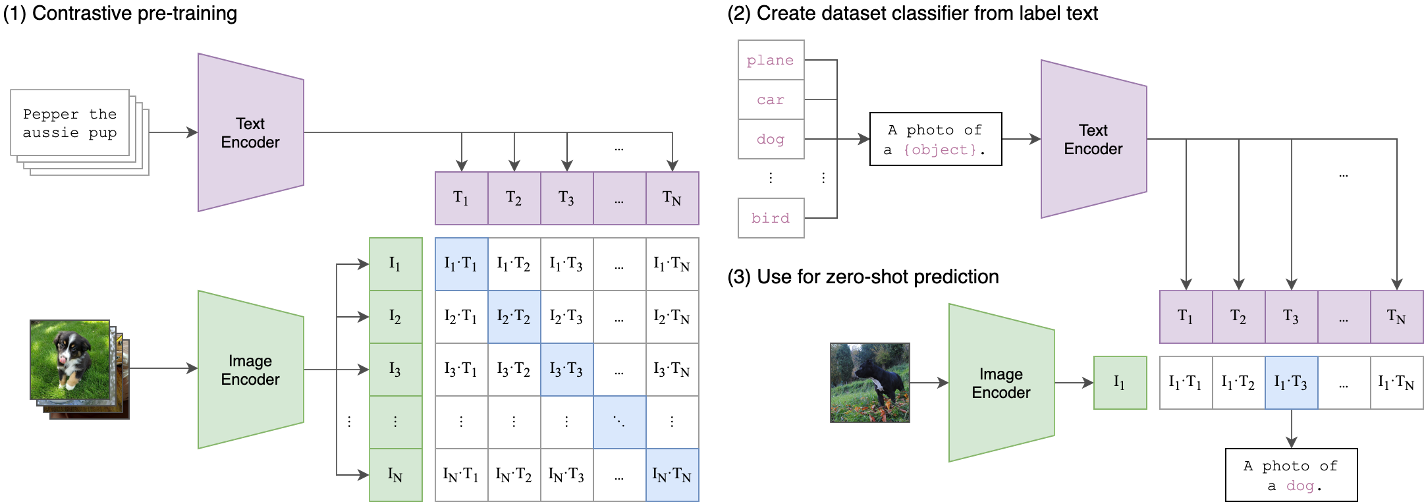
\includegraphics[scale=0.5]{CLIP_structure}
	\caption{CLIP model summary.}
	\label{fig:figure3}
\end{figure}

Because of the inability to change parameters and adjust the model, it will be excluded from the comparison to the other techniques.
The other algorithms used will be explained within the Methods section.

\subsection{Hypothesis}
Between the three animals, we expected to see Pandas being the most accurately predicted class since they are always Black and White, and have high contrast in fur.
This is especially true when compared to dogs and cats, which can come in a variety of colored fur.
Furthermore, we expected the Neural Network Algorithms as well as the pre-trained algorithms to perform faster and more accurately than SVM.
  \graphicspath{ {project_images/} }

\section{Methods}

We implemented the SVM, CNN, ResNet50, and VGG16 classifiers in our project as the algorithms of interest.
Below, we will describe the algorithms used in detail.

\subsection{SVM}
SVM operates by defining a division line between classes using a kernel function. 
The chosen kernel function, uses parameters $C$ and $\gamma$ to perform the calculation to separate the dataset into their respective classes \cite{SVMExplained, SVMExplained2}.
In our case, we converted the images to arrays to allow SVM to process our dataset.
Before feeding the dataset, it is imperative to have the dataset standardized.
We decided to standardize it using MinMaxScaler, as StandardScaler would change the data to be within the range $[0,1]$ and took extra time to process, while ultimately yielding no significant improvement in performance of the constructed model.
By implementing a Pipeline, we were able to consolidate the code and concisely read the process being done by the program.
Also, by using GridSearch, we were able to let the SVM classifier run with a K-Fold comparison added to find the best performing model.

\begin{figure}[h]
	\centering
	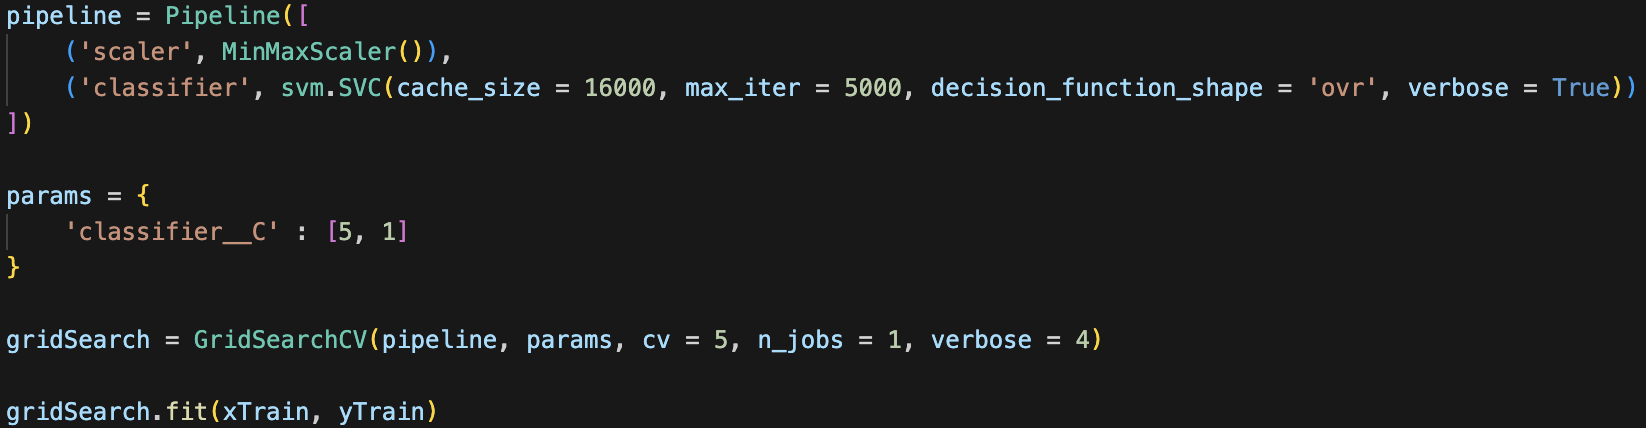
\includegraphics[scale=0.3]{SVM_explained.png}
	\caption{SVM using Pipeline and Grid Search within the Jupyter Notebook}
	\label{fig:figure2}
\end{figure}

\subsection{CNN}
Convolutional Neural Networks (CNN) are commonly used for image classification tasks. 
Typically, CNN models consist of convolutional layers that apply filters to extract features and patterns, pooling layers to retain the important features and patterns, and fully connected layers to make predictions based on the features learned in the convolutional and pooling layers \cite{CNNGuide}.
Our CNN model implements a sequential structure, where the layers are added linearly. 
The input layer takes in the parameters of the image, in our case our images were 500 pixels by 500 pixels with a color channel of 1 (since they are greyscale images). 
After input, the first convolutional layer applies filters to capture the features in the image data by moving a matrix of learnable weights over the image. 
In our model, the filters had a size of 3x3 and the number of filters increased in each convolutional layer. 
The weights are randomized before training and begin updating their value throughout the training process. 
The extracted features are put into a feature map that the following pooling layer uses to further extract important features. 
Our model uses max-pooling, which looks for the maximum value extracted by each filter from the previous layer so that the initial feature map is downsampled. 
This pattern of convolutional layer followed by pooling layer iterates to continue extracting features and downsampling the feature map before applying a flatten layer.
This reshapes the feature map into a one-dimensional vector that can be inputted into a fully connected dense layer. 
The convolutional layers and max-pooling layers iterate 3 times in our model before the feature map is flattened. 
We found that less iterations yielded poorer performance (underfitting) and more iterations resulted in longer training time (model was more complex and computational load was larger). 
The dense layer is considered a "fully connected" layer because each neuron in a dense layer is connected to every extracted feature and is assigned a weight value. 
The weight of each of the connections in the dense layer attempt to understand the relationship between the important features extracted from the previous layers as a representation of a prominent feature. 
The output layer is a dense layer with neurons equal to the number of classes in the dataset; in our case there are 3 classes (cat, dog, and panda). 
The summary of the structure of our CNN model is shown in Figure \ref{fig:figure3} below.

\begin{figure}[h]
	\centering
	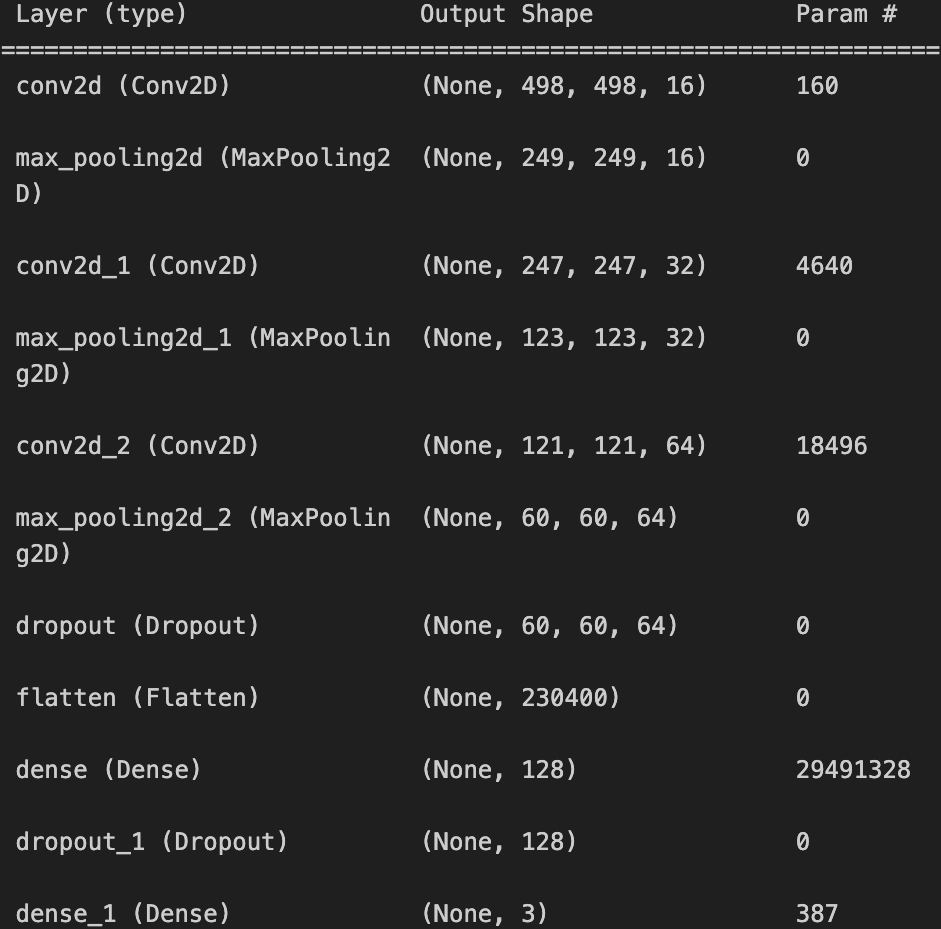
\includegraphics[scale=0.5]{CNN_structure}
	\caption{CNN model summary.}
	\label{fig:figure3}
\end{figure}

%INSERT CITATION(s) SOMEWHERE IN THIS PARAGRAPH FOR THE INFO DISCUSSING DROPOUT/RELU
%the citatino should be number 15
Our convoluted layers use the Rectified Linear Unit (ReLu) activation function to introduce non-linearity, this way our model can learn complex relationships between the features of our data. 
The ReLu activation function sets negative values found in the convolution matrix to 0, allowing the model to focus on the positive values that likely represent relevant features. 
In between the dense layers, we implemented dropout regularization to prevent overfitting. 
Dropout works by temporarily setting the weights of a random set of neurons to 0 ("dropping out") per epoch. 
This prevents overfitting by forcing the model to learn more robustly instead of relying too much on the recognition of certain features and "memorizing" the training data. 
The output dense layer uses the Softmax activation function to scale the numerical output of the model into probabilities distributed over the possible output classes represented by indexes. 
The class with the highest probability is considered the predicted class which is mapped to the string value of the class using the index value.

While fitting the model, we implemented the EarlyStopping callback to reduce the likelihood of overfitting by stopping training if the validation accuracy did not improve after 5 consecutive epochs. 
The EarlyStopping callback can also be useful in preventing underfitting if the number of epochs is set to a higher number than what is expected to be necessary. 

\subsection{ResNet50}

Residual Network 50 (ResNet50) is a type of CNN algorithm that contains 50 hidden layers. 
This algorithm allows for the use of Convolution2D and MaxPooling2D layers just like the standard CNN algorithm.
The 'Residual' portion refers to how the gradient is handled within the structure of the algorithm itself.
The gradient is the result calculated from the partial derivatives of the loss function, with respect to the given data's parameters \cite{Gradient}.
Instead of using standard back-propogation, it has a separate structure called a residual block which allows for the gradient to flow more easily through the entire structured network\cite{RN50}.

\begin{figure}[h]
	\centering
	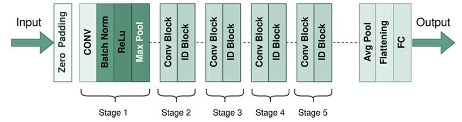
\includegraphics[scale=0.5]{ResNet_structure.jpg}
	\caption{A sample structure of the Res Net 50 Algorithm}
	\label{fig:figure4}
\end{figure}

\newpage

\subsection{VGG16}
VGG16 is a pre-trained CNN model available for use through Tensorflow. 
VGG16 was pre-trained for image classification on large datasets such as ImageNet where the input image size was 224 pixels by 224 pixels with 3 color channels (RGB). 
Its structure consists of 13 convoluted layers and 3 fully connected dense layers (16 layers total) \cite{VGG16Explained}. 
We decided to use a pre-trained VGG16 model instead of building one from scratch to learn how efficiently it would execute our particular image classification task. 
To utilize the pre-trained VGG16 model, we first load the base model without the top layers as these layers are what we need to modify to have the model classify our cat, dog, and panda images. 
Initially, the custom layers we added included 3 fully connected dense layers.
However, we found the training time to be especially long and after experimenting with removing a dense layer to make the model less complex, we found that the training time was shortened with very little change in performance. 
Ultimately, we chose to keep working with the shortened training time with two dense layers. 
The first dense layer utilizes ReLu activation as well as the He uniform kernel initializer to initialize the weights of the 64 neurons within a uniform range dependent on the number of input neurons. 
The He uniform combats the possibility of too many dead neurons by increasing the likelihood that neurons will activate and not be stuck in an inactive state throughout the entirety of training. 
This gives more neurons the chance to contribute to learning. 
The structure of the pre-trained VGG16 is shown in Figure \ref{fig:figure5} below. 
The last output dense layer acts the same as it did in our previous CNN model, utilizing Softmax to generate probabilities distributed over the three output classes mapped to their corresponding string values. 

\begin{figure}[h]
	\centering
	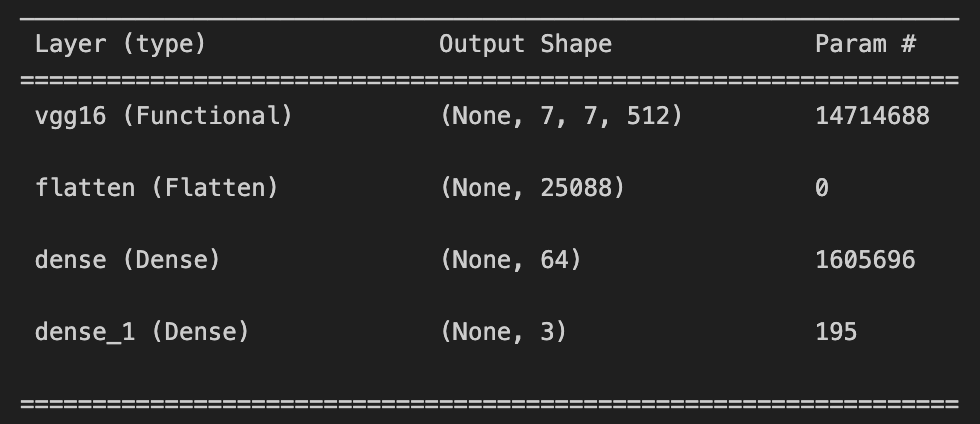
\includegraphics[scale=0.5]{VGG16_structure}
	\caption{Pre-trained VGG16 model summary. The base model is loaded and the top dense layers are added manually.}
	\label{fig:figure5}
\end{figure}
  \section{Evaluation}
[Evaluate and compare the models performance]
Evaluation: Compare the methods you used
  \section{Conclusions}
Here you summarize the essential aspects and findings 
of your work and analysis.

Finally, remember to include a section with the bibliography.
It is very important to cite the sources you used for your study and
for writing the report.

    % bibliography / References

  \begin{thebibliography}{}

    \bibitem{AIAdv} \href{https://ai100.stanford.edu/gathering-strength-gathering-storms-one-hundred-year-study-artificial-intelligence-ai100-2021-1/sq2#:~:text=In%20the%20last%20five%20years,and%20integration%20of%20vision%20and}{Stanford: What are the most important Advances in AI?}

    \bibitem{publicOpinion} \href{https://www.pewresearch.org/short-reads/2023/08/28/growing-public-concern-about-the-role-of-artificial-intelligence-in-daily-life/}{PRC: Growing public concern about the role of artificial intelligence in daily life}
  
    \bibitem{Dataset} \href{https://www.kaggle.com/datasets/ashishsaxena2209/animal-image-datasetdog-cat-and-panda}{Kaggle: Animal Image Dataset(DOG, CAT and PANDA)}

    \bibitem{SVM} \emph{Comparison of Support Vector Machine Classifier and Naïve Bayes Classifier on Road Surface Type Classification} by Marianingsih and Utaminingrum.

    \bibitem{CNNPerformance} \emph{How Does the Data set Affect CNN-based Image Classification Performance?} by Luo, Li, Wang, et. al.

    \bibitem{AnimalSpecies1} \emph{An Enhanced Animal Species Classification and Prediction Engine using CNN} by Priya, Kalyan, et. al.
  
    \bibitem{AnimalSpecies2} \emph{Animal Species Image Classification} by Prudhivi, Krishna et. al.

    \bibitem{AnimalBreed} \emph{Animal Breed Classification and Prediction Using Convolutional Neural Network Primates as a Case Study} by Kamepalli, Kolli, and Bandaru

    \bibitem{Mosquito} \emph{CNN Architectures Performance Evaluation for Image Classification of Mosquito in Indonesia} by Amiruddin and Kadir

    \bibitem{CLIP} \href{https://github.com/openai/CLIP/tree/main}{CLIP algorithm Github Page}

  \end{thebibliography}

\end{document}